\chapter{Evaluation}

The solution is now in its completion. It can produce a battle system that,  according to itself, is well-balanced. In this chapter we will try to validate if humans agree with this claim or not.

\section{Evaluate a battle system for balance}

\subsection{Methodology}
\label{sub:meth}

In order to evaluate the solution, first we ran the solution to generate a battle system with balance as the objective. We then picked another system, evaluated to make sure that according to the same evaluation criteria, it was not as balanced as the generated one. Then we let human volunteers play the game on both systems, without telling them which one was generated, and asked them a series of questions to identify which system they thought was more balanced.

\subsubsection*{Balanced system}

To produce a balanced battle system, the genetic algorithm part of the solution was run, using the following configurations:
\begin{itemize}
	\item Population size is 50.
	\item Stop GA process after no better solution could be found for 30 generations. (Maximum generation is 500, but this is irrelevant.)
	\item Use min-max as the top-level fitness combinator, to combined the 4 major objectives.
	\item Simulate 50 battles for each matchup in each generated battle system.
	\item A battle ends as a draw if no clear winner emerges after 200 turns.
\end{itemize}

The process was run twice, producing two different `best' systems (because of inherent randomness in the GA process). The one with the lower fitness was chosen. Figure \ref{fig:systemj} shows the entire run that produced this system, with the best fitness of 0.2.

\begin{figure}
	\centering
	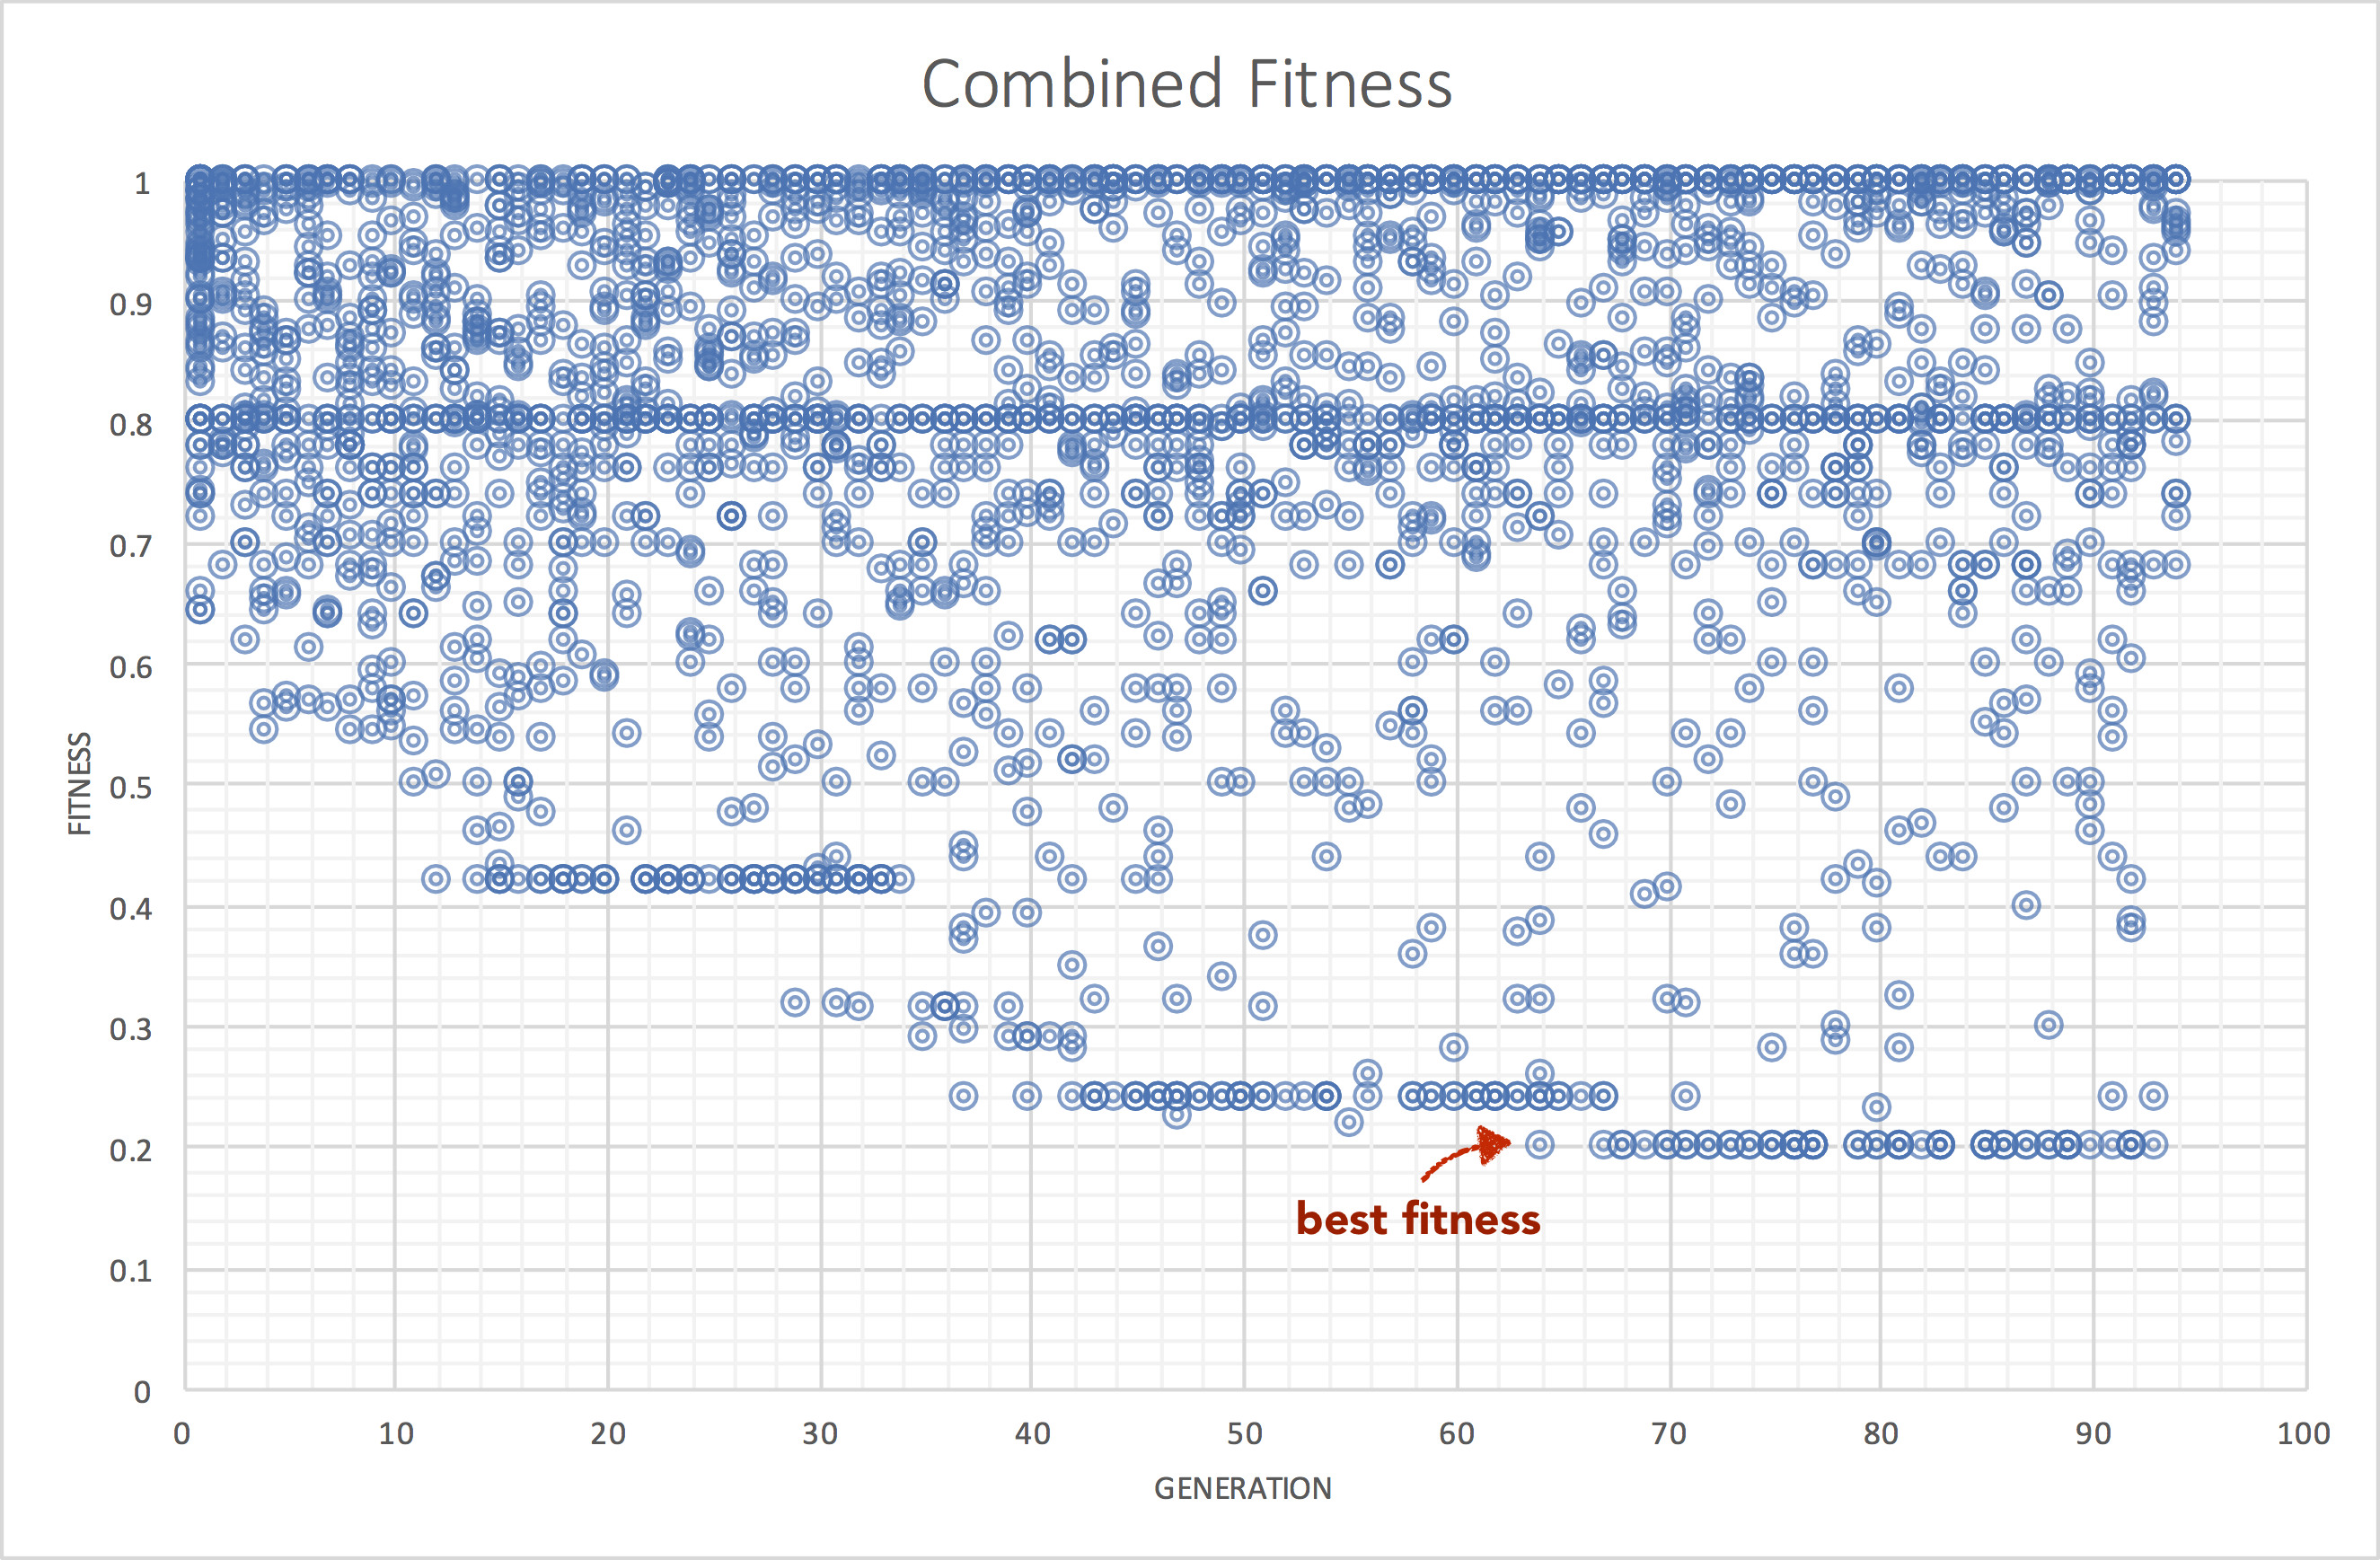
\includegraphics[width=0.8\linewidth]{figures/j-ga}
	\caption{The fitness of all generated battle systems, with respect to the combined objective, in the GA run that produced the system to be used in evaluation.}
	\label{fig:systemj}
\end{figure}

We then used the result of this run as a starting population for subsequent runs, in which the top-level fitness combinator was changed from \textit{min-max} to \textit{weighted average} and \textit{weighted-normalised geometric mean}. Comparing the results, it is not obvious which combinator produce the best result, as the best systems reported by these combinators all exist on the \textit{Pareto front} -- a set of points such that there exist no other point that is better than them in all dimensions\cite{marler2004survey} (see figure \ref{fig:combinators}). Any of these systems can be chosen as the generated balanced system, and we chose  the original system produced by the \textit{min-max} combinator.

\begin{figure}
	\centering
	\begin{subfigure}{0.6\textwidth}
		\centering
		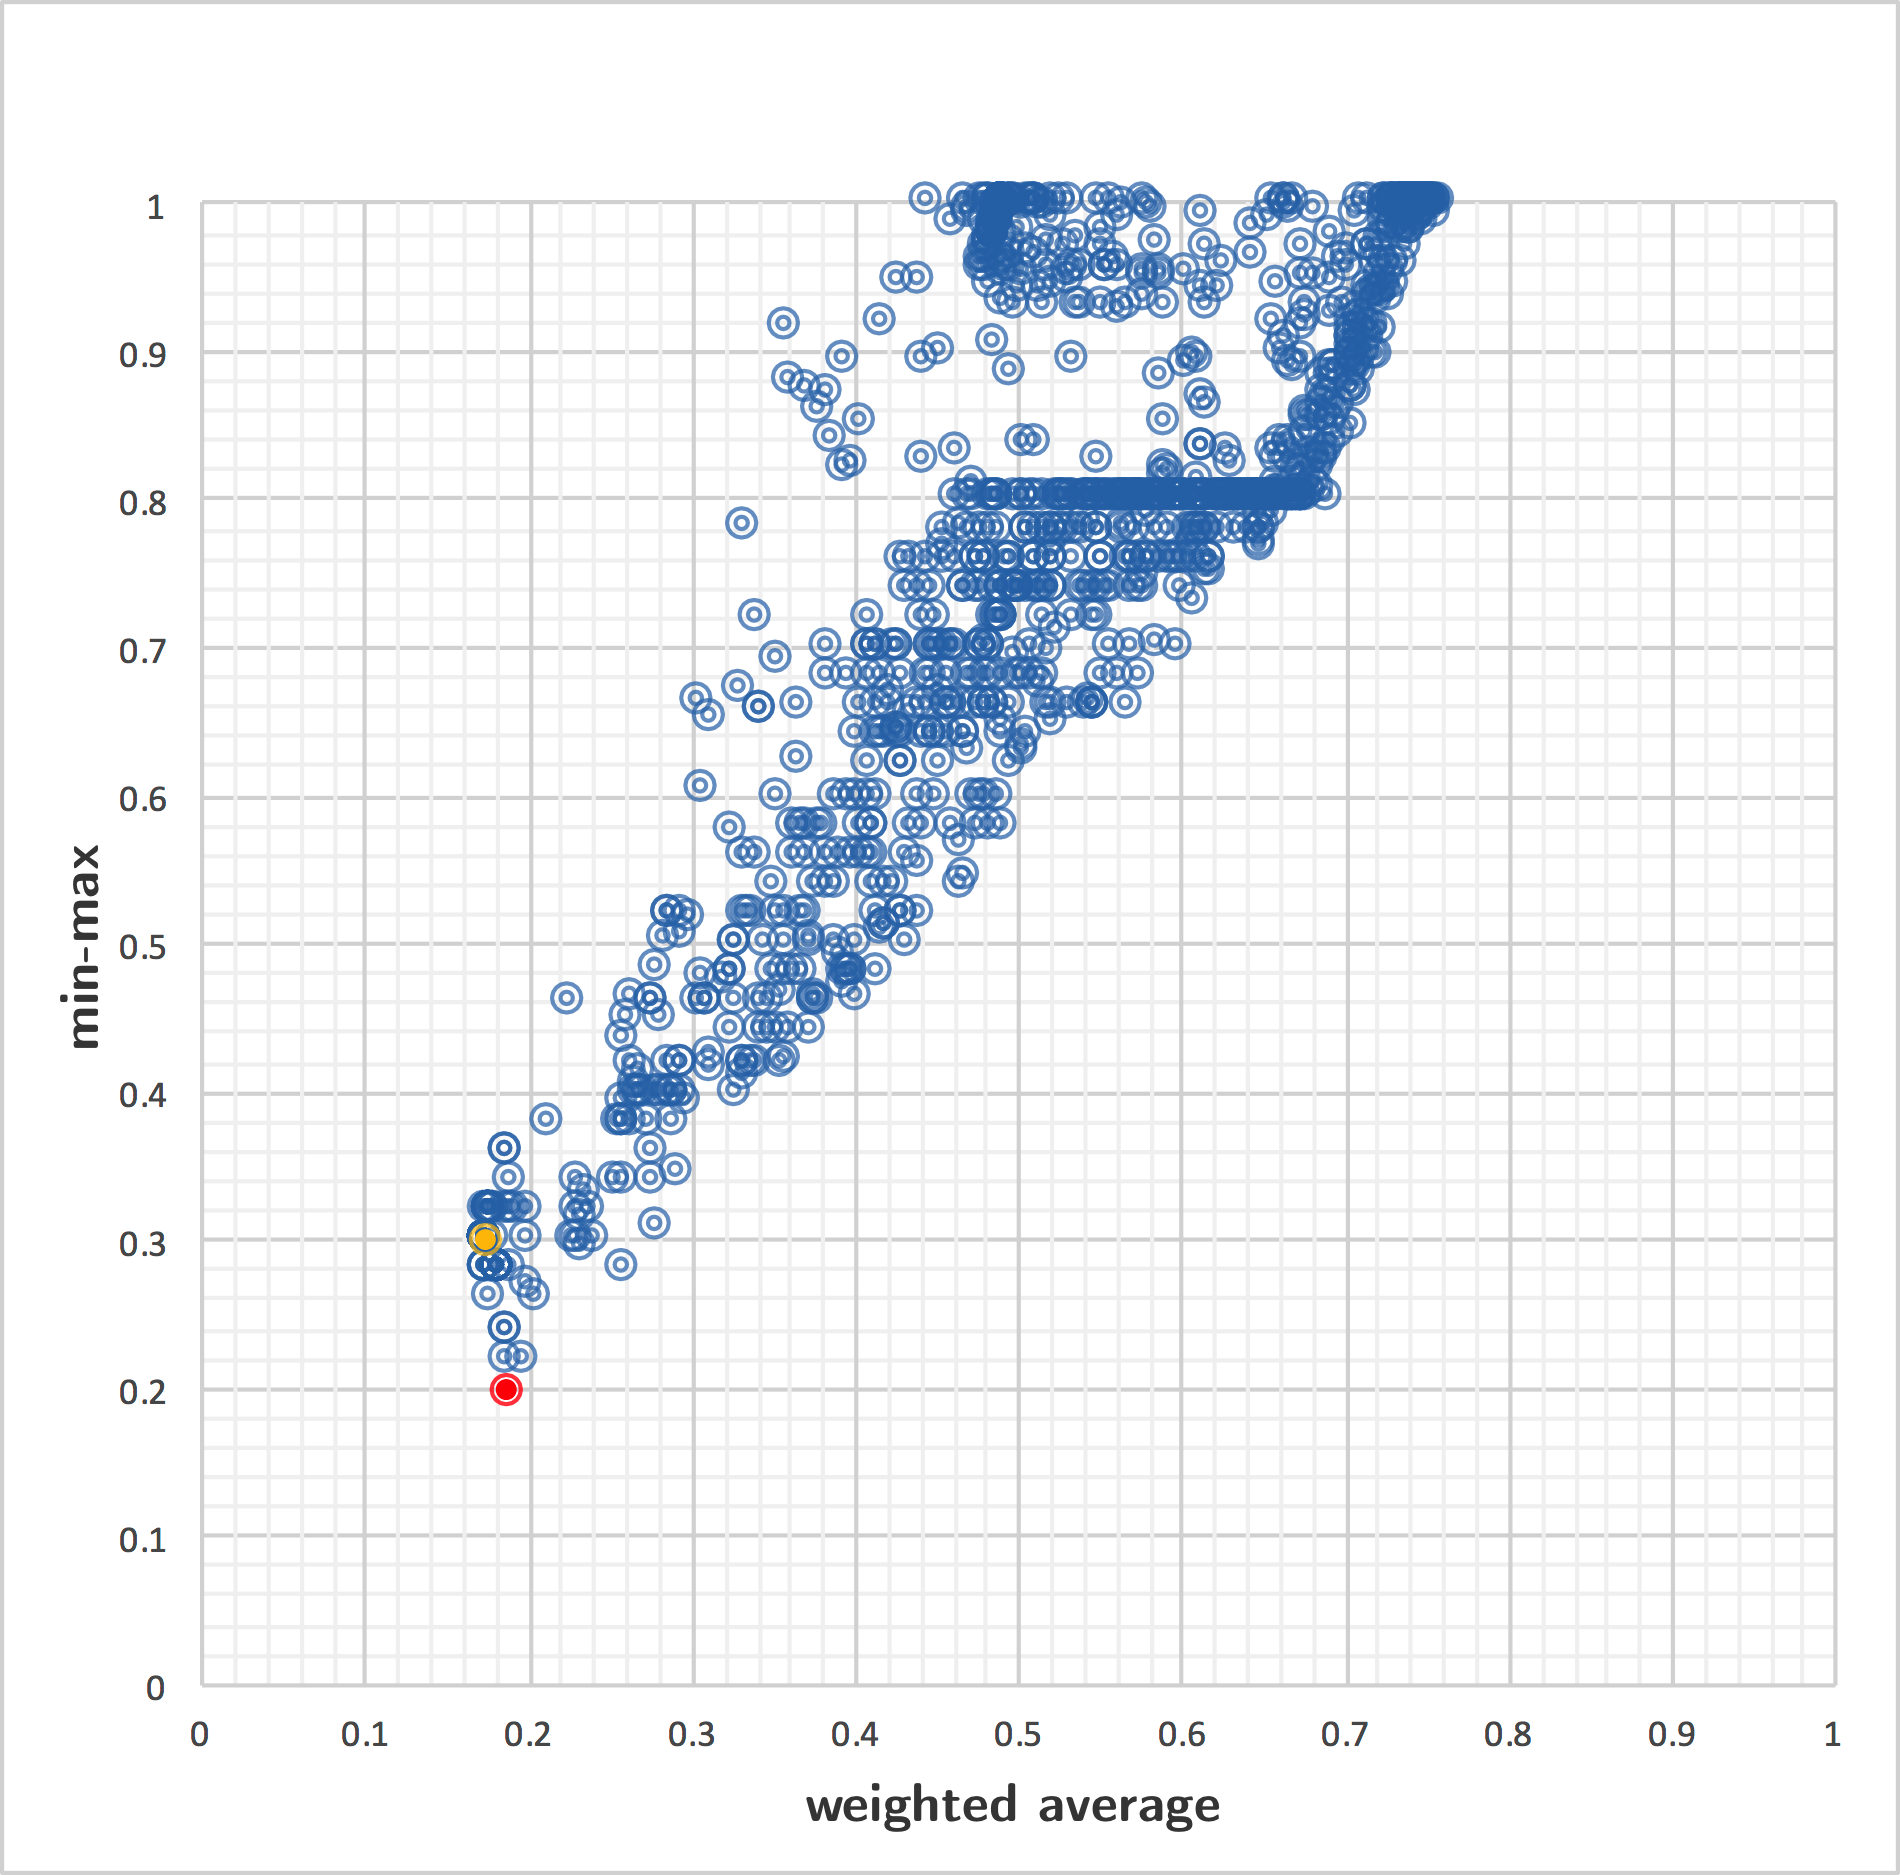
\includegraphics[width=1\linewidth]{figures/combinator_max_sum}
		\caption{Weighted average}
	\end{subfigure}
	\begin{subfigure}{0.6\textwidth}
		\centering
		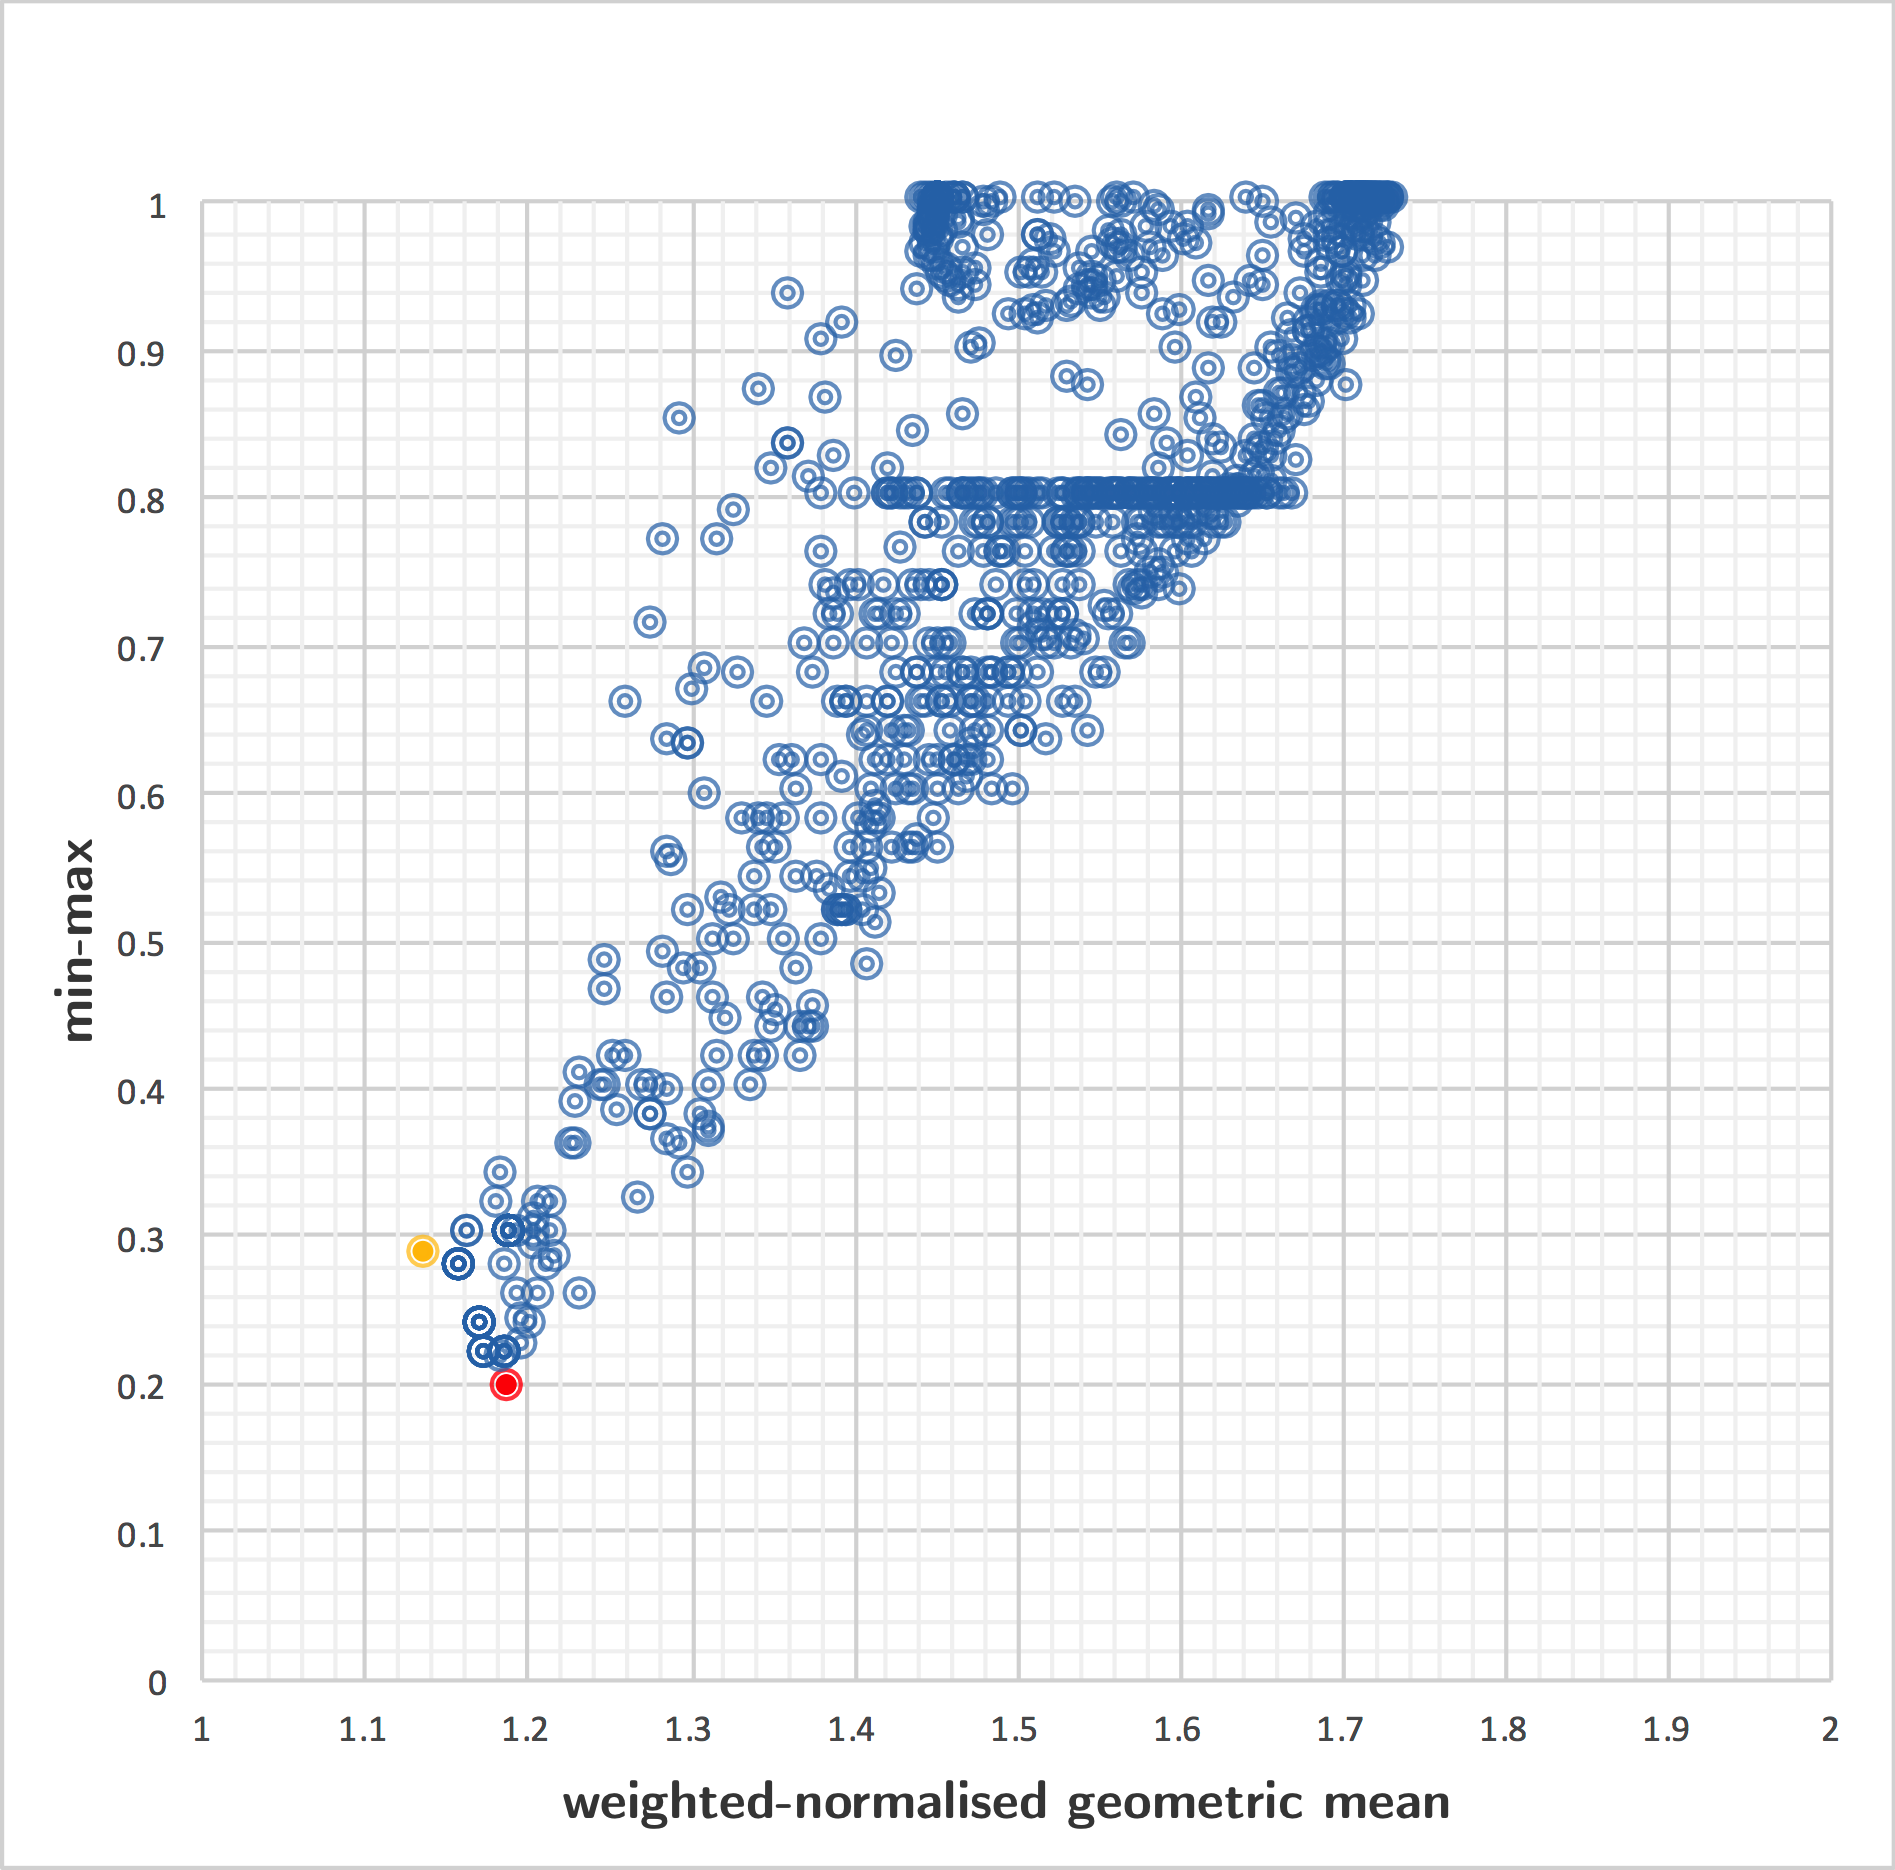
\includegraphics[width=1\linewidth]{figures/combinator_max_prod}
		\caption{Weighted-normalised geometric mean}
	\end{subfigure}
	\caption{Combinators comparison. The red points have the best fitness, according to \textit{min-max} combinator. The orange points are the best as reported by \textit{weighted average} and \textit{weighted-normalised geometric mean} combinators.}
	\label{fig:combinators}
\end{figure}

\subsubsection*{Unbalanced system}

The experiment needs another system to be compared with the generated one. We simply used the manually-created preliminary system that was recovered, as explained in section \ref{sub:recovery}.

We named the generated system as `system J', and the manually created system as `system H'. In table \ref{table:compare_hj} the objective fitnesses of the two systems are compared against each other, and also against another randomly generated system\footnote{The configuration for testing the two systems were: number of battles = 1000, battles are drawn at number of turns = 1000, random seed = 0. The random system was selected  from the starting populations of the two GA runs in the previous section, using the one whose min-max fitness is at the median.}. It can be seen that, in all the fitness combinators we have tried, the generated system is the most balanced, followed by the manually-created system, which is still more balanced that a random system.

\begin{table}
	\begin{tabu}{X[l5] X[c2] X[c2] X[c2]}
		\toprule
		objective & System J & System H & random\\ 
		\midrule
		\ warrior > ranger & 0.060 & 0.266 & 0.800\\
		\ ranger > mage & 0.018 & 0.200 & 0.720\\
		\ mage > warrior & 0.195 & 0.794 & 0.200\\
		\textbf{combat triangle} & 0.195 & 0.794 & 0.800\\
		\ anyone > cleric & 0.093 & 0.100 & 0.080\\
		\ team+cleric > team & 0.267 & 0.389 & 0.260\\
		\textbf{clerics as supporters} & 0.267 & 0.389 & 0.260\\
		\textbf{no first-mover advantage} & 0.008 & 0.015 & 0.060\\
		\textbf{appropriate damage} & 0.267 & 0.794 & 0.935\\
		\midrule
		combined (min-max) & 0.267 & 0.794 & 0.935\\
		combined (wgt. average) & 0.202 & 0.579 & 0.712\\
		combined (wgt. normalised geometric mean) & 1.199 & 1.557 & 1.683\\
		\bottomrule
	\end{tabu}
	\caption{Comparison of each sub-objective on systems J, H, and random.}
	\label{table:compare_hj}
\end{table}

\subsubsection*{User study}

The two systems were tested by human testers. We asked our 10 volunteers to download the solution and play around with the prototype, using both battle systems H and J. They were not told how these two systems are different. After that we asked them to fill out a questionnaire revolving around the feeling of balance. Full instruction and questionnaire can be found in appendix \ref{app:questionnaire}.

The respondents are:
\begin{itemize}
	\item mostly male (80\%)
	\item aged between 23-34 years old
	\item play games often (60\% play on a daily basis)
	\item quite familiar with the genre of tactical RPG (60\%)
\end{itemize}

\subsection{Results}

First we asked if the prototype can be classified as a TRPG game. Most (70\%) agreed, the rest said they were not sure.

We then proceeded to the main purpose of this user study -- to confirm that the battle system generated from the solution is more balanced than the one created manually. This was asked in a few different ways.

\subsubsection*{Direct question}

\begin{figure}
	\centering
	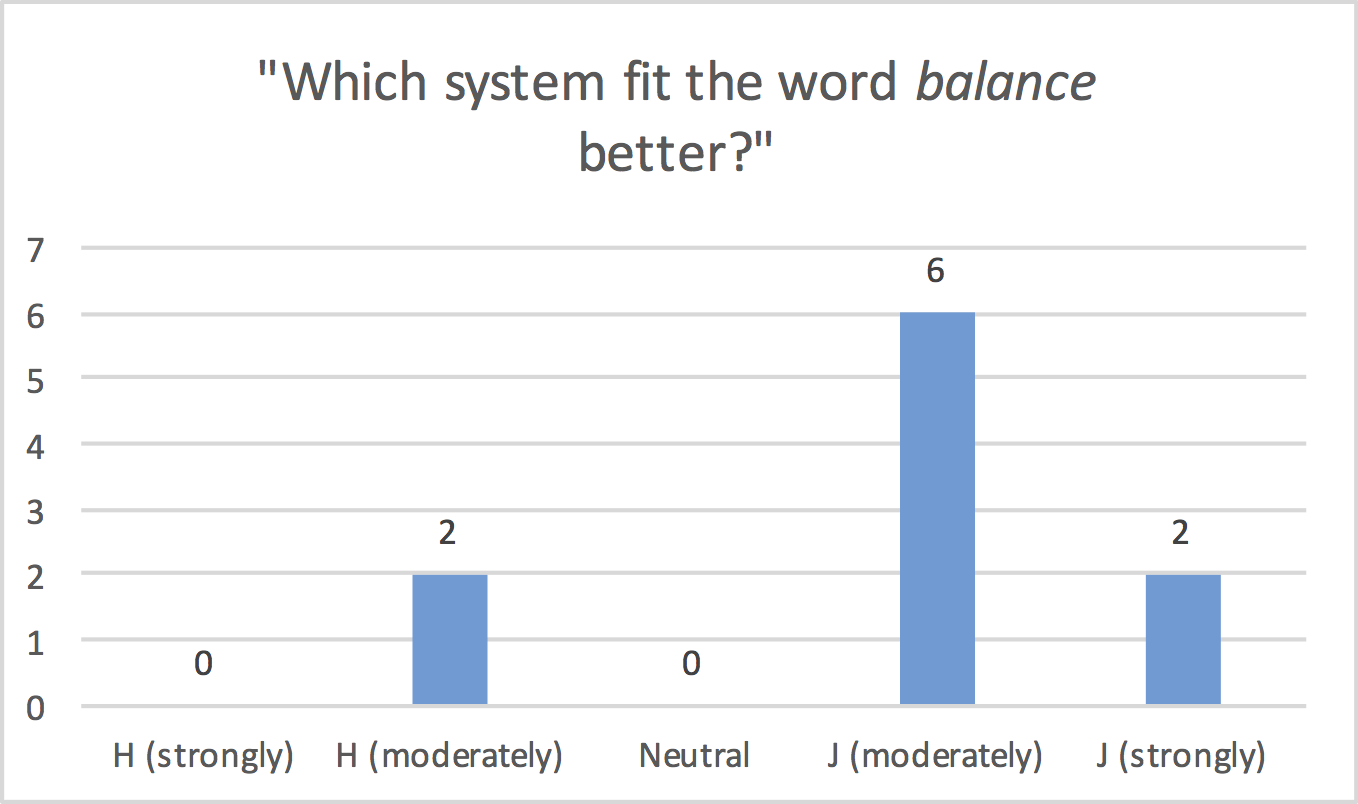
\includegraphics[width=0.6\linewidth]{figures/bar_balanced}
	\caption{Result of associating `balance' with the battle systems.}
	\label{fig:result_bar_balance}
\end{figure}

One of the question asks the respondents directly how they associate the term `balance' with the two battle systems. The result is as in figure \ref{fig:result_bar_balance}: 8 out of 10 respondents associated `balance' with the generated system, with 2 of them said the association is strong.

\subsubsection*{Balance as in `not overpowered'}

As noted in earlier chapters, there is no consensus on the precise definition of the word `balance'. Our interpretation is that a balanced system should not allow any unit to be too `overpowered' -- being able to beat all other units. The combat triangle was design according to this interpretation. The questionnaire did not define `balance', and thus it is possible that the volunteers might have a different interpretation than ours.

\begin{figure}
	\centering
	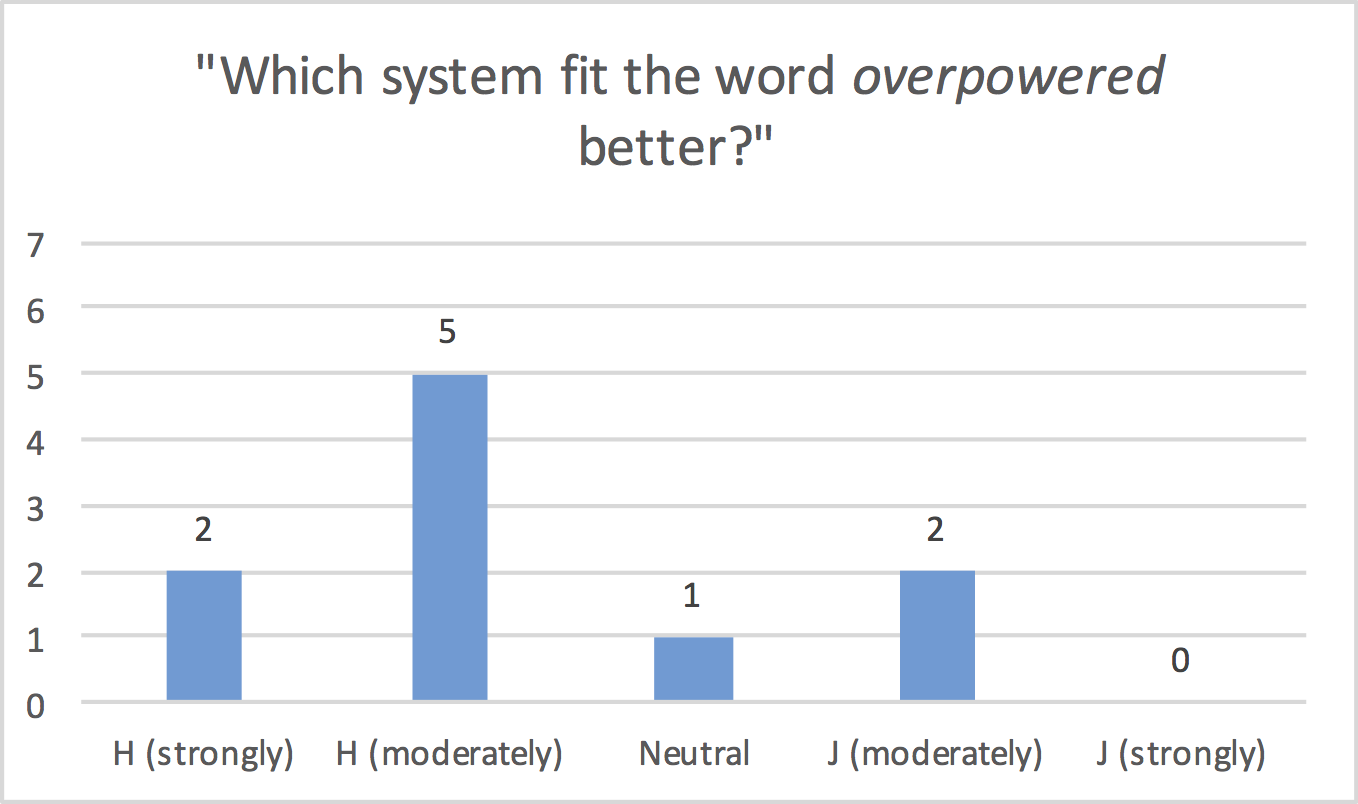
\includegraphics[width=0.6\linewidth]{figures/bar_op}
	\caption{Result of associating `overpowered' with the battle systems.}
	\label{fig:result_bar_op}
\end{figure}

For this reason, in addition to `balance', the respondents were also asked to associate `overpowered' with the two systems. The result is as in figure \ref{fig:result_bar_op}: 7 out of 10 respondents associated `overpowered' with the manual system, whereas 2 chose the generated system. This is a positive result -- the generated system is less overpowered.

As an anecdote, this does not necessarily mean that the respondents agree with our definition of balance. One of them said the generated system is \textit{both balanced and overpowered}, while another stated the opposite -- choosing the manual system for both characteristics. Investigating further, the responses were assign scores, as follows:
\begin{itemize}
	\item 1 for `System J (strongly)'
	\item 0.5 for `System J (moderately)'
	\item 0 for `Neutral'
	\item -0.5 for `System H (moderately)'
	\item -1 for `System H (strongly)'
\end{itemize}
It was then found that the correlation between \textit{balance} and \textit{overpowered} is merely -0.142, suggesting a weak negative relationship, while we expected a much stronger one.

\subsubsection*{Fun factor}

In addition to `balance' and `overpowered', respondents were also asked to associated `fun', `fast-paced', and `challenging' with the two systems. Using the same score assignment aforementioned, the correlation between `fun' and the others are:
\begin{itemize}
	\item Balance: 0.853
	\item Fast-paced: 0.829
	\item Overpowered: -0.010
	\item Challenging: -0.172
\end{itemize}

While this is not the result needed for differentiation of the two battle systems, it does justify our claim that \textit{balance is important for the enjoyment of the game}.

\subsubsection*{Party selection}

The questionnaire further asked the respondents to assemble a party of 4 units, choosing a combination of jobs that would be most likely to beat an AI party consists of one unit for each of the four jobs. We observed the following:

\begin{figure}
	\centering
	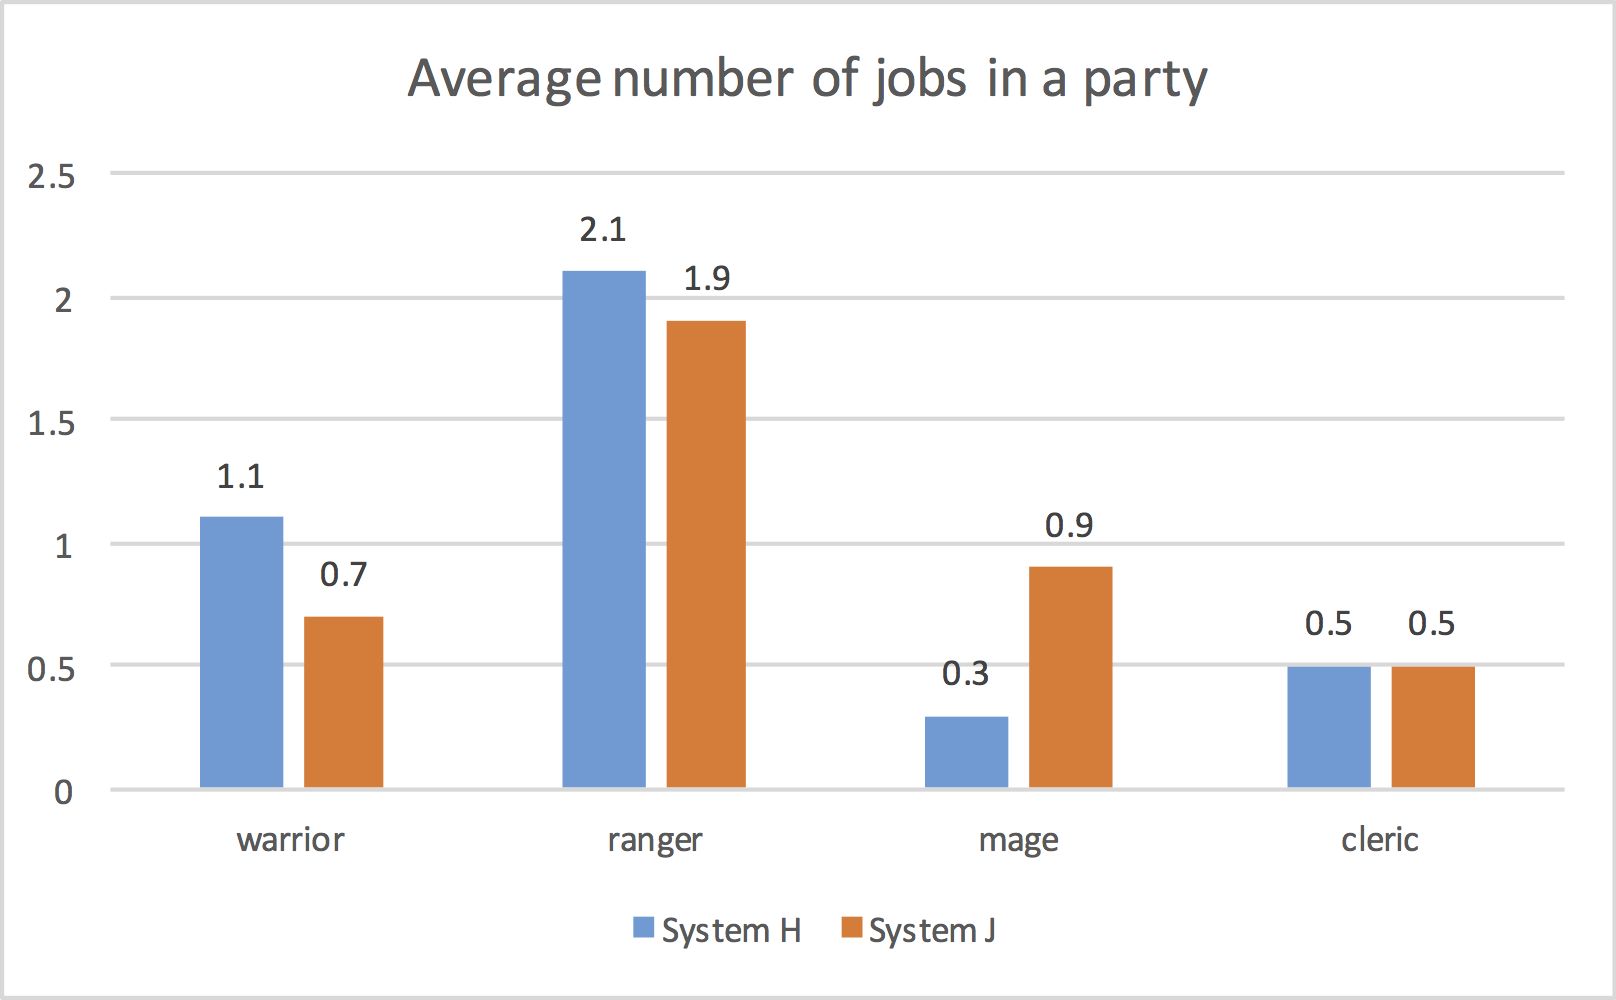
\includegraphics[width=0.6\linewidth]{figures/jobs_per_party}
	\caption{Distribution of jobs in the respondent-assembled parties.}
	\label{fig:jobs_per_party}
\end{figure}

\begin{itemize}
	\item For the three attacking character classes, the respondents perceived rangers to be the strongest by far, followed by warriors, then mages. This is true for both battle systems, but the disparity is more pronounced in the manually-created system than the generated one, as seen in figure \ref{fig:jobs_per_party}.
	
	\item We hypothesised that if a respondent can feel the presence of the combat triangle, then the assembled party should have at least one unit from each of the three attacking jobs. For system H (the manually-created one), only 1 out of 10 party qualifies for this criterion. System J does just a little better, with 2 qualified parties, but still far from what we expected from a balanced system. 
	
	Another hypothesis is that if the clerics-as-supporters objective is achieved, then the assembled party should consist of exactly one cleric. For both battle systems, half of the parties qualified for this criteria.
	
	Comparatively, the difference in the battle systems has no observable effect to the way the parties are assembled.
	
	\item An interesting fact is that, for 4 out of 10 respondents, their assembled parties for both battle systems are \textit{exactly the same}, despite them having clear distinction between the two systems, given their answers to other questions. This suggests that the perception of balance might not affect the party selection in the way we expected -- there could be other factors in the party formation decision (such as personal preferences to certain character classes).
\end{itemize}

In the end, we could not draw any conclusive result from this part of the questionnaire.

\section{Threats to validity}

This section identifies the threats to the validity of our results.

\begin{itemize}
	\item \textbf{Small size of respondents.} The number of respondents is 10. From statistical point of view, small sample size reduces the confidence level of the result.
	\item \textbf{Use of a single battle system to represent the solution.} The solution can produce a lot of battle systems. We generated a few and picked what we thought of as the best one for evaluation. This only proves (if the validation is justified) that the solution can generate a good battle system, but does not say anything about quality of battle systems produced by the solution in general.
\end{itemize}

\section{Summary}

In this section we evaluated the solution to the research question, by generating a battle system with the goal of balance, then asked a number of volunteers to compare it against an unbalanced system, without telling them which is which. Overall, most (70\%--80\%) of the 10 respondents agreed that \textbf{the generated system is more balanced and less overpowered}, even though the two terms are not as strongly correlated as we thought. However, balance does strongly imply enjoyment, justifying our position of using it as the optimisation goal. Contrary to our hypotheses, the perception of balance cannot be easily judged by how the players assemble their party. Finally we identified some threats that could undermine the validity of our result.